\section{Gamma}
La distribuzione Gamma generalizza le distribuzioni esponenziale e chi--quadro. 
Essa coincide con la distribuzione della somma di $\alpha$ variabili aleatorie indipendenti e identicamente distribuite, ciascuna con legge esponenziale di parametro $\beta$, con $\alpha > 0$ e $\beta > 0$.


\[
\Gamma(\alpha,\beta)
\]

\begin{figure}[H]
\centering

% ===================== PDF =====================
\begin{minipage}{0.45\textwidth}
\centering
\begin{tikzpicture}
\begin{axis}[
    axis lines = middle,
    ylabel = {$f(x)$},
    xlabel = {$x$},
    width = 0.90\textwidth,
    height = 0.90\textwidth,
    ymin = 0, ymax = 1.2,
    xmin = -0.5, xmax = 10
]

% --- Gamma(alpha=1, beta=1) ---
\addplot[black, thick, domain=0:10, samples=400]
{exp(-x)};

% --- Gamma(alpha=2, beta=1) ---
\addplot[gray!60, thick, domain=0:10, samples=400]
{x*exp(-x)};

% --- Gamma(alpha=2, beta=2) ---
\addplot[dashed, thick, domain=0:10, samples=400]
{(2^2)*x*exp(-2*x)};

\end{axis}
\end{tikzpicture}
\end{minipage}
\hfill
% ===================== CDF =====================
\begin{minipage}{0.45\textwidth}
\centering

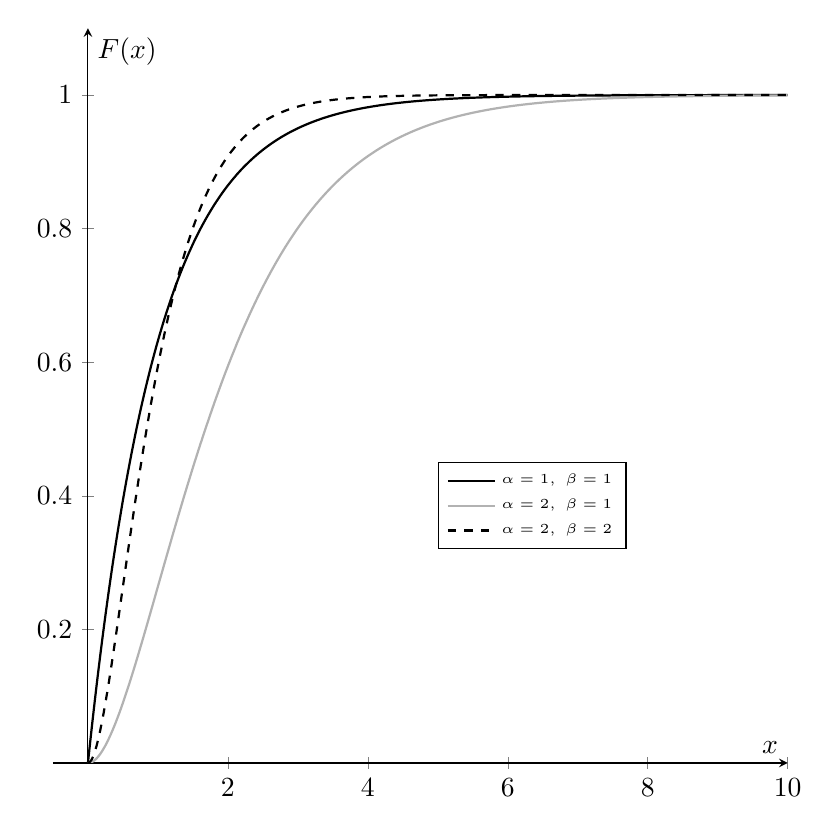
\begin{tikzpicture}
\begin{axis}[
    axis lines = middle,
    ylabel = {$F(x)$},
    xlabel = {$x$},
    width = 0.90\textwidth,
    height = 0.90\textwidth,
    ymin = 0, ymax = 1.1,
    xmin = -0.5, xmax = 10,
    legend style={at={(axis cs: 5,0.45)}, anchor=north west, font=\tiny},
    legend cell align=left,
]

% --- CDF Gamma(alpha=1, beta=1) ---
\addplot[black, thick, domain=0:10, samples=400]
{1 - exp(-x)};
\addlegendentry{$\alpha=1,\ \beta=1$}

% --- CDF Gamma(alpha=2, beta=1) ---
\addplot[gray!60, thick, domain=0:10, samples=400]
{1 - exp(-x)*(1 + x)};
\addlegendentry{$\alpha=2,\ \beta=1$}

% --- CDF Gamma(alpha=2, beta=2) ---
\addplot[dashed, thick, domain=0:10, samples=400]
{1 - exp(-2*x)*(1 + 2*x)};
\addlegendentry{$\alpha=2,\ \beta=2$}

\end{axis}
\end{tikzpicture}

\end{minipage}


\end{figure}

\bigskip
\begin{table}[H]
\centering
\renewcommand{\arraystretch}{2}
\begin{tabular}{@{}ll@{}}
\toprule
\textbf{Supporto} 
& $[0,+\infty)$ \\

\midrule

\textbf{Funzione di Densità} 
& $
f(x)=
\dfrac{\beta^\alpha}{\Gamma(\alpha)}
x^{\alpha-1}\,e^{-\beta x}\;\mathbb{I}_{(0, +\infty)}(x)
$ \\

\midrule

\textbf{Funzione di Ripartizione}
& $
F(x)=
\dfrac{\gamma(\alpha,\beta x)}{\Gamma(\alpha)}
\qquad
\bigl(\text{dove }\gamma \text{ è la gamma incompleta inferiore}\bigr)
$ \\

\midrule

\textbf{Valore atteso} 
& $\mathbb{E}[X]=\dfrac{\alpha}{\beta}$ \\

\midrule
\textbf{Momento $\boldsymbol{k}$--esimo}
& $\mathbb{E}\left[X^k\right] = \dfrac{\beta^\alpha}{\Gamma (\alpha)} \dfrac{\Gamma(\alpha + k)}{\beta^{\alpha + k}}$ \\

\midrule

\textbf{Varianza}
& $Var(X)=\dfrac{\alpha}{\beta^2}$ \\

\midrule

\textbf{Funzione caratteristica}
& $
\varphi_X(u)=
\left(\dfrac{\beta}{\beta-iu}\right)^{\alpha}
$ \\

\bottomrule
\end{tabular}
\end{table}


\noindent Si ricorda che la funzione Gamma di Eulero è definita, per ogni $\alpha>0$, come
\[
\Gamma(\alpha)=\int_{0}^{+\infty} x^{\alpha-1} e^{-x}\,dx,
\]
e generalizza il fattoriale al continuo, nel senso che
\[
\Gamma(n)=(n-1)! \qquad \forall n\in\mathbb{N}.
\]
